\documentclass[a4paper]{article}
\usepackage{iwslt15,amssymb,amsmath,epsfig,placeins}
\setcounter{page}{1}
\sloppy		% better line breaks
%\ninept
%SM below a registered trademark definition
\def\reg{{\rm\ooalign{\hfil
     \raise.07ex\hbox{\scriptsize R}\hfil\crcr\mathhexbox20D}}}

%% \newcommand{\reg}{\textsuperscript{\textcircled{\textsc r}}}

\title{Football Prediction}

%%%%%%%%%%%%%%%%%%%%%%%%%%%%%%%%%%%%%%%%%%%%%%%%%%%%%%%%%%%%%%%%%%%%%%%%%%
%% Please make sure to keep technical paper submissions anonymous  !
%%%%%%%%%%%%%%%%%%%%%%%%%%%%%%%%%%%%%%%%%%%%%%%%%%%%%%%%%%%%%%%%%%%%%%%%%%
%\name{}
%%%%%%%%%%%%%%%%%%%%%%%%%%%%%%%%%%%%%%%%%%%%%%%%%%%%%%%%%%%%%%%%%%%%%%%%%%
%% If multiple authors, uncomment and edit the lines shown below.       %%
%% Note that each line must be emphasized {\em } by itself.             %%
%% (by Stephen Martucci, author of spconf.sty).                         %%
%%%%%%%%%%%%%%%%%%%%%%%%%%%%%%%%%%%%%%%%%%%%%%%%%%%%%%%%%%%%%%%%%%%%%%%%%%
\makeatletter
 \def\name#1{\gdef\@name{#1\\}}
 \makeatother
 \name{{\em David Monschein, Marius Dörner}}
%%%%%%%%%%%%%%% End of required multiple authors changes %%%%%%%%%%%%%%%%%

\address{Final Report for Praktikum Neuronale Netze WS18/19 \\
Karlsruhe Institute of Technology}
%
\begin{document}
\maketitle
%
\begin{abstract}
Predicting the outcome of football games is interesting to a lot of people, from
football enthusiasts to people working in the betting industry. It is also an
interesting research problem, due to its complexity and difficulty, because even
humans can not precisely predict the outcome of soccer games. In the Praktikum
we used data about past matches, including teams and their players, to train
different types Neural Networks. We created a simple fully connected Network and
a bit more complex Network which uses a Long-short-term-memory architecture.
Afterwards we evaluated them regarding their accuracy and compared the results.
\end{abstract}
%
\section{Introduction}
In the last few years, neural networks became increasingly more popular and were
applied to a wide range of problems in different fields, e.g. in computer
vision, natural language processing or speech recognition. In this project we
studied the application of neural networks to a more unusual task, namely to
predict the outcome of football matches. More precisely, given the data of two
football teams we had to predict the outcome of a match between them, i.e.
either predict the winner or predict if the game ends in a draw. \\
For development we used the \emph{European Soccer Database} \cite{1} which
contains more than 25.000 professional football matches and statistics for 299
teams and their associated players collected over multiple seasons from various
European soccer leagues like the German Bundesliga, the English Premier League
and the Spanish Primera División. \\
For this project, we developed two neural network models: A feed-forward model
and a recurrent neural network (RNN) model. We compare their performance against
bookmaker predictions on the same matches. \\
This report is organized as follows: Section \ref{data} describes the structure
of our dataset, the features we used as input for our networks and our data
loading procedure. Section \ref{models} introduces our  models and their
training procedures. Section \ref{experiments} describes our experimental setup
and presents our results. We conclude our work in Section \ref{conclusion}.

\section{Related Work} \label{relatedwork}
There are a lot of existing machine learning approaches which deal with
predicting football games.
\\\\
The creator of the database used a Support Vector Machine (SVM) to predict the
football matches. He stated that his approach is able to classify 53\% of the
matches correctly \cite{SVM-Kaggle}. But it has to be said that there is no
information about the evaluation process, so the accuracy of around 53\% is not
confirmed.
\\\\
Andrew Carter presented an approach which uses a Deep Neural Network (DNN) based
on Tensorflow \cite{DeepLTensor}. He was able to achieve an accuracy of 51\% and
in addition he developed a betting strategy that can be used in combination with
his DNN approach.
\\\\
There are plenty of other machine learning projects which address the prediction
of soccer games \cite{MLFramework1, MLFramework2}. The methods used within these
projects vary greatly, they used a lot of different evaluation methods and
metrics, so it is not possible to compare them directly.

\section{Data} \label{data}
The data we used has been published on Kaggle and is called the ``European
Soccer Database''\footnote{https://www.kaggle.com/hugomathien/soccer/}. As the
name suggests, it contains information about the outcome of past football games.
The data is provided as an SQLite database with several tables. The next
sections introduce the coarse structure of the database and explain which
challenges arised while dealing with the data.

\begin{figure*}[!htbp]
	\centering
    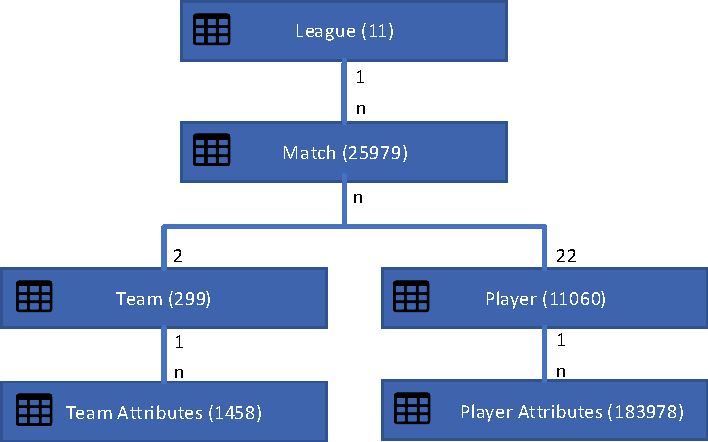
\includegraphics[scale=0.8]{img/table-layout-nn}
	\caption{Tables and their relations in the used SQLite database}
	\label{fig:data}
\end{figure*}

\subsection{Structure}
The SQLite database holds data about 11 different leagues. Summed up, it
consists of around 26000 matches of 299 teams. For each match it contains all
players that started in this match, for both the home team and the away team.
Furthermore there are attributes for all teams, which quantify the properties of
a certain team. An example for such an attribute is the overall rating of a
team, it is a value between 0 and 100 and approximates how good a team is.
Similar to the team attributes the database contains information about 36
different attributes for each player (e.g.
rating, shot power, \ldots). The team attributes and the player attributes are
documented at different timestamps, so the database respects teams and/or
players which get better or worse over time. During the preprocessing we select
the attribute sets with the smallest time difference to the considered match. It
is important that only attributes are used which are known before the match
begins.
\\\\
The attributes were extracted from the video game
FIFA\footnote{https://www.easports.com/de/fifa}.
Figure \ref{fig:data} shows a simplified view of the tables in the SQLite
database.

\subsection{Challenges}
We encountered two problems during the preprocess tasks. The first problem is
related to a lot of missing attributes and obviously wrong values. The second
problem is caused by unbalanced data. The home team statistically wins in 44\%
of all cases, therefore the database contains much more matches that are labeled
with a home win in comparision with draws and away wins.
\subsubsection{Incomplete Data}
The three major challenges, due to inaccurate and incomplete data, were:
\begin{enumerate}
  \item Entirely missing player IDs $\rightarrow$ The only possible solution to
  deal with this is ignoring the matches because the given data is not
  sufficient to predict a football game reasonably.
  \item A small subset of player IDs are missing $\rightarrow$ We applied
  different strategies. The ones that worked the best were inserting default
  values and using aggregated values for the player attributes (min, max, avg,
  deviation, \ldots).
  \item Missing player attributes $\rightarrow$ The problem is similar to the
  missing player IDs for a match. The possible solutions are the same,
  aggregations and inserting default values worked the best.
\end{enumerate}
We tried different approaches for dealing with this inaccuracies and selected
the ones that worked the best. For missing player IDs we introduced a
``default'' player with attributes that are equal to the average of all other
players in the team. With missing player attributes we dealt in the same way, we
infered default values.

\subsubsection{Unbalanced Data}
As already mentioned, the home team wins statistically about 44\% of all
matches. The away team wins 30\% of the matches and the remaining 26\% are
draws. We do not want to introduce a bias so it was necessary to balance the
data in the preprocess phase.
\\\\
We used \textbf{undersampling} to realize this. That means we removed around
14\% of the home wins to balance the data. However, in the evaluation phase we
recognized that the impact of balancing the data is negligible.

\subsection{Preprocessing}
Querying the needed the data from the SQLite database on every startup was very
slow and also introduced the overhead of preprocessing prior to the training.
Therefore we decided to query the needed data once, preprocess it and write it
back to a CSV file. The main advantage of this approach is that we do not need
to run queries against the database before training, which makes the startup
significantly faster.
\\\\
We split up the data in 80\% Training and 20\% Test. The Training data was
seperated in 85\% pure Training data and 15\% Validation data. We implemented a
dataset which conforms to the PyTorch Dataset structure that allows us to use
existing features of the PyTorch framework (e.g. batching).

\section{Method} \label{models}
We developed two models that are based on the \textit{Siamese Network} approach
\cite{Bromley94} which is extensively used for tasks that require to find
similarities between two inputs, a recent example for this is \textit{Facenet}
\cite{Schroff15} a face recognition model. In our case we are given the data of
two football teams and need to predict the outcome of a match between them,
basically a comparison task. Teams are represented as a matrix $T \in
\mathbb{R}^{11 \times m}$ where the row $T_i$ contains the attributes of the
$i$-th player of a given team. We denote the \textit{away team} with $T^a$ and
the \textit{home team} with $T^h$. Note that we only consider the eleven
starting players for each team as we don't have data for substitute players. A
description of the player attributes is given in Section \ref{data}.

\begin{figure} 
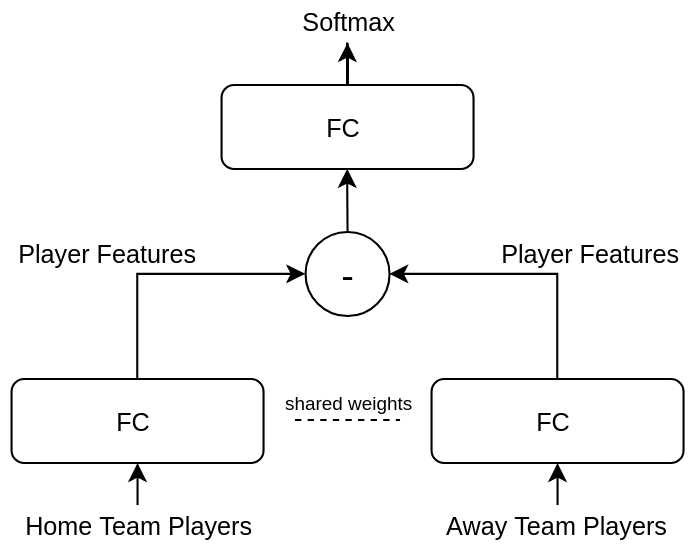
\includegraphics[scale=0.30]{img/Siamese1.png}
\caption{First model for match outcome prediction.}
\label{fig:ffnet}
\end{figure}

\subsection{Fully Connected Model}
Our first model consists of two fully connected neural networks as depicted in
Figure \ref{fig:ffnet}. The first network learns an embedding $f(T) \in
\mathbb{R}^d $ for the team data. We use this network for both teams during a
forward pass, which means that the weights for the inputs are shared during the
backwards pass. Given the features $f(T^h)$ and $f(T^a)$ for the home and away
team we use the difference $f(T^h)-f(T^a)$ as the input for the second network,
which predicts the probabilities $p_h, p_d, p_a$ for home win, draw and away win
using the Softmax activation function in the output layer. For the inner layers
we use the ReLU (rectified linear unit) activation function. We also use
\textit{Dropout} \cite{Dropout14} layers with probability $0.1$ in both
networks. The layers for the team embedding are depicted in Table
\ref{tab:flayer} and the layers for the prediction network are depicted in Table
\ref{tab:player}.
 
\begin{table}
\begin{tabular}{|c|c|c|c|}
\hline 
\textbf{Layer} & \textbf{Input Size} & \textbf{Output Size} & \textbf{Activation} \\ 
\hline 	
\hline
linear1 & $11 \times 35=385$ & $128$ & ReLU \\ 
\hline 
linear2 & $128$ & $128$ & ReLU \\ 
\hline 
dropout1 & $128$ & $128$ &  \\ 
\hline 
\end{tabular} 
\caption{Feature layers for the FC model.}
\label{tab:flayer}
\end{table}

\begin{table}
\begin{tabular}{|c|c|c|c|}
\hline 
\textbf{Layer} & \textbf{Input Size} & \textbf{Output Size} & \textbf{Activation} \\ 
\hline 	
\hline
linear1 & $128$ & $128$ & ReLU \\ 
\hline 
linear2 & $128$ & $128$ & ReLU \\ 
\hline 
dropout1 & $128$ & $128$ &  \\ 
\hline 
linear2 & $128$ & $3$ & Softmax \\ 
\hline
\end{tabular} 
\caption{Prediction layers for the FC model.}
\label{tab:player}
\end{table}

\subsection{Match Histories}
Our first model only considered data from a single game but football teams play
on a weekly basis during a season and performance over the last couple of games
may be predictive of performance in future matches because of influences that
are hard to measure numerically e.g. how competent a teams coach is in picking
strategies or how good a team fits together on an interpersonal basis. For our
second model we want to consider this additional information for both teams
during the prediction but we first need to extract this from the dataset. \\
For the performance of a team we consider the goal differences of past matches
from the teams point of view, e.g. if Team A wins $3$ to $1$ against Team B then
the goal difference from Team As' point of view is $2$ whereas the difference
from Team Bs' point of view is $-2$. Thus the goal difference of a draw is $0$
for both teams. Given a team and a date we call the series of goal differences
of this teams past matches in this season up to the given date its \textit{match
history}. For example a team that played three matches with outcomes $3$ to $1$,
$2$ to $3$ and $0$ to $0$ has the match history $(2, -1, 0)$. Note that we only
consider games that were played in the same season, we don't go over seasons
boundaries as professional football teams often change considerably during the
off season (buying and selling players, new coaches etc.). We also want to
emphasise here that match histories have different lengths depending on their
end date, e.g. at the first matchday of a new season no team has a history yet
while on the last matchday each team has a full season worth of games in its
history (in most leagues around $30$ games). Thus the length of the match
history is variable during the seasons and we need to consider that while
building our model. \\
We can construct match histories efficiently using only one pass over our
dataset if all matches in a season are ordered by their match dates (ordering
between seasons does not matter). We iterate over the matches by ascending date
and create a buffer data structure, e.g. a Python deque,  for each 'new' team we
encounter, this buffer holds all the row indices of the past matches of its team
in the dataset. For each match entry we add the current buffer content of both
teams as a new column. Basically, each match now contains an list of dataset
indices that reference the past matches (other rows in the dataset) of both
teams. We implemented this using the PyTorch dataset class but this could also
be implemented with other frameworks, for example using Pandas DataFrames.

\begin{figure} 
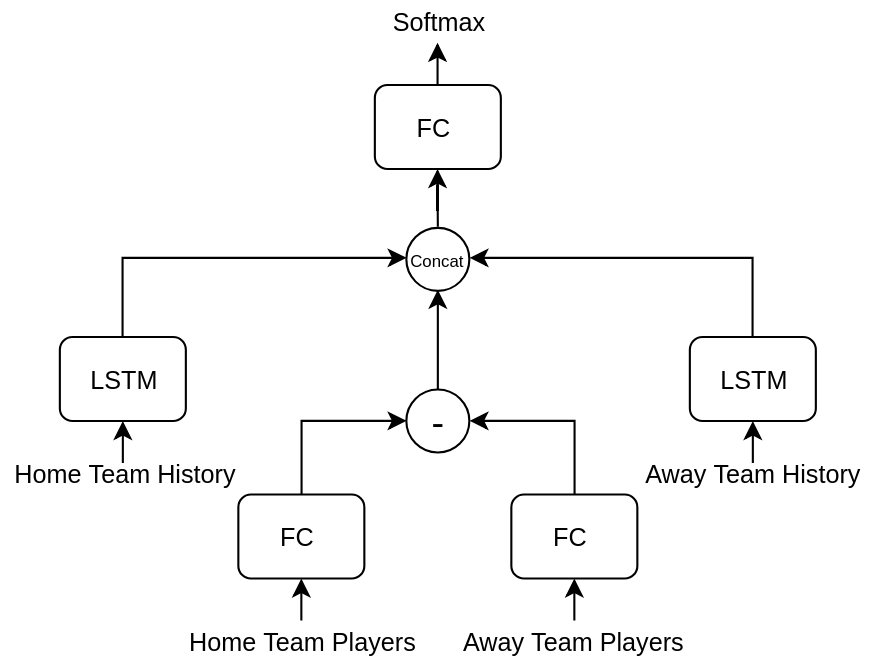
\includegraphics[scale=0.28]{img/Siamese2.png}
\caption{Second model for match outcome prediction.}
\label{fig:rnn}
\end{figure}

\subsection{RNN Model}
For our second model we want to use the match histories as additional
information. As we already described that match histories have different lengths
at different match dates a recurrent neural networks seems fitting for use as a
match history encoder. We again use the player data $T^a$ and $T^h$ in the same
way as in the fully connected model, that is we use the network described in
Table \ref{tab:flayer} to learn embeddings $f(T^a)$, $f(T^h)$ for the away and
home team and input the difference $f(T^h) - f(T^a)$ into the prediction
network. For the recurrent neural network we use a LSTM \cite{LSTM97} with one
hidden layer with $32$ neurons. As a goal difference is a single number we use a
Linear Layer with shape $1 \times 32$ and Tanh activation before the LSTM. We
feed the series of goal differences completely into the LSTM and use its last
hidden state as an additional input for our prediction network. Note that there
are matches for which the match history is empty, i.e. at the start of a season,
in these cases we don't use the LSTM at all and only use the predictions from
the fully connected model.\\
Similar to the fully connected network we use same LSTM (but reinitialize its
hidden state after the first team) to encode the match histories of the teams
which means that its weights are also shared for both inputs during training. \\
The input of the prediction network is the difference between the team
embeddings $f(T^h) - f(T^a)$ concatenated with the last hidden states of the
LSTMs for both match histories. The prediction network is the same as in the
first model (Table \ref{tab:player}) but with a larger input size ($192$ instead
of $128$) in its first layer to account for the additional inputs.

\section{Experiments} \label{experiments}
\subsection{Setup}
We implemented our models using the PyTorch framework \cite{PyTorch} and trained
them on Googles
\textit{Colab}\footnote{https://research.google.com/colaboratory} service which
provides free access to a Nvidia K80 GPU. Our training data was found on Kaggle
as described in Section \ref{data}.

\begin{figure} 
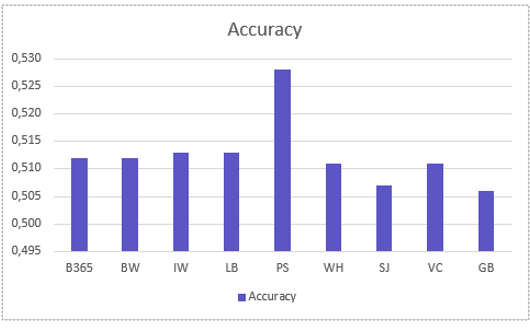
\includegraphics[scale=0.40]{img/bmacc.png}
\caption{Prediction accuracy for different bookmakers in our dataset as evaluated on the test set. Average accuracy for bookmakers is 0.513.}
\label{fig:bmacc}
\end{figure}

\subsection{Bookmaker Predictions as Baseline}
For nearly every match in our dataset \textit{odds} from various bookmakers,
online services where people can bet on the outcome of football matches, were
included. Bookmakers denote odds $o_h, o_a, o_d \in \mathbb{R}_{\geq 1}$ for
each possible outcome, i.e. home win $o_h$, away win $o_a$ and draw $o_d$ which
can basically be seen as multipliers for the returns on successful bets, e.g.
betting 10 euro on an outcome with 1.5 odds returns 15 euros on a win. To make a
profit or break even a bookmaker needs to set the odds in a way that reflects
the outcome of a match, e.g. the most likely outcome should have the lowest odds
and thus the lowest payout from the bookmakers point of view and so on.
Therefore the odds actually represent the bookmakers predictions w.r.t. the
match outcome and in theory there is even an inverse relationship between
probabilities and odds, $p_x = 1/o_x$, but in practice bookmakers actually
decrease the odds to add a profit margin for themselves, a process called
\textit{fixing the odds}. A more thorough review of bookmaker mathematics is out
of the scope for this document, even though we can still assume that the odds in
our database reflect which outcome the bookmakers believed to be most likely, as
they would probably still assure that this one is the most "unattractive" to bet
on. \\
For these reasons we use the predictions given by the odds as baseline to
compare our models against. We evaluated their predictions on the matches in our
test set using an ensemble of nine different bookmakers. Their results are shown
in Figure \ref{fig:bmacc}, the mean prediction accuracy is 0.513.

\begin{figure} 
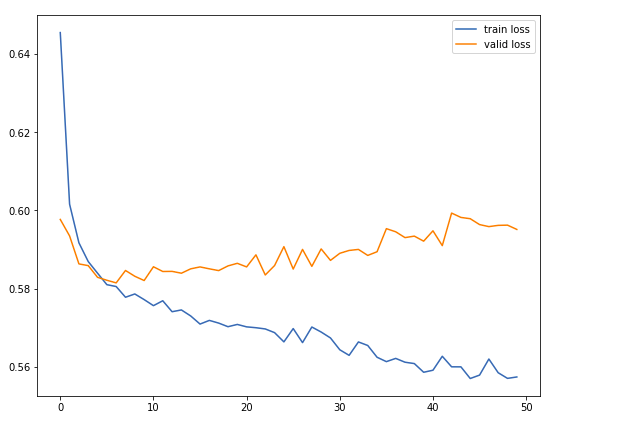
\includegraphics[scale=0.35]{img/experiment1.png}
\caption{Training loss for the fully connected model. }
\label{fig:fcloss}
\end{figure}
\begin{figure} 
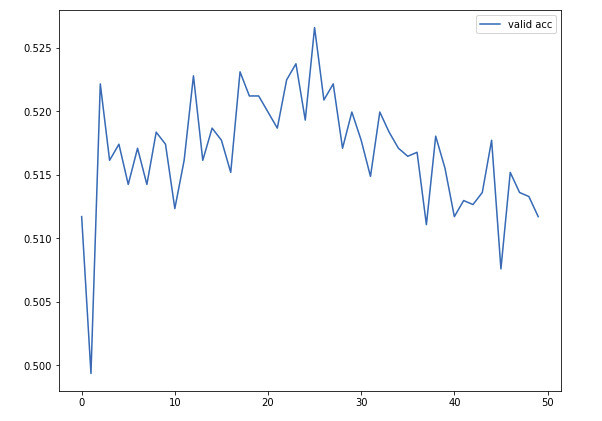
\includegraphics[scale=0.35]{img/acc1.png}
\caption{Validation accuracy for the fully connected model. }
\label{fig:fcacc}
\end{figure}

\begin{figure} 
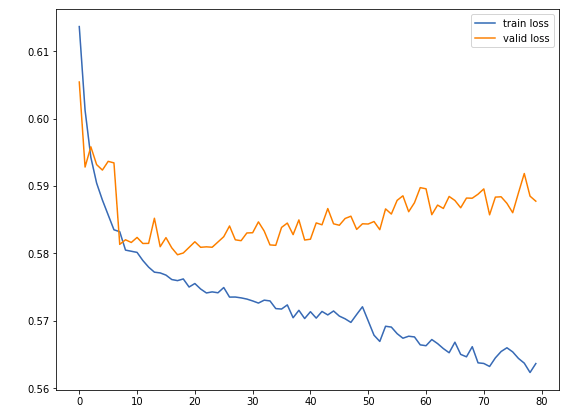
\includegraphics[scale=0.35]{img/loss2.png}
\caption{Training loss for the recurrent model. }
\label{fig:rnnloss}
\end{figure}
\begin{figure} 
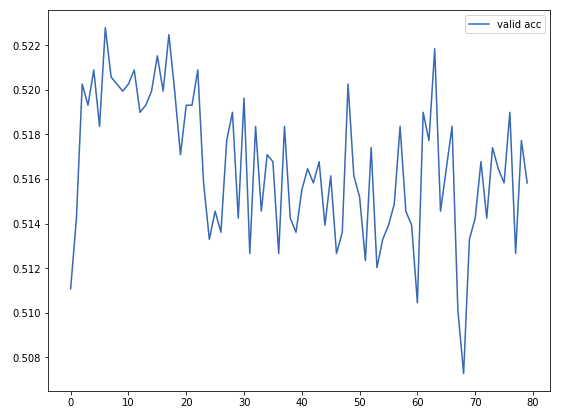
\includegraphics[scale=0.35]{img/acc_exp2.png}
\caption{Validation accuracy for the recurrent model. }
\label{fig:rnnacc}
\end{figure}



\subsection{Training}
We train both of our models with the cross entropy loss function. Our fully
connected model was trained with the Adam \cite{Adam} optimizer with a learning
rate of $0.0025$ and a batch size of $1024$. The training loss and validation
accuracies for this models are shown in Figure \ref{fig:fcloss} and
\ref{fig:fcacc}. We see that this models tends to overfit quickly even with
small learning rates so we only trained it for five epochs for our evaluation.
\\
For our recurrent model we only batch sizes of $32$ matches as the variable
length match histories we consider here have to either be padded or cut
accordingly so that each match in the mini batch has histories of the same
length. As padding is problematic here, e.g. padding with zeros would mean to
add additional draws to the match history, we cut them on the same length for
each match, so small batch sizes reduce the amount of cutting needed. The model
was trained using the PyTorchs' SGD optimizer with a learning rate of $0.01$ and
$0.01$ momentum. Loss curves and validation accuracies for the recurrent model
are shown in Figures \ref{fig:rnnloss} and \ref{fig:rnnacc}. This models also
starts to overfit after some time, so for evaluation we stopped training after
30 epochs.

\begin{figure} 
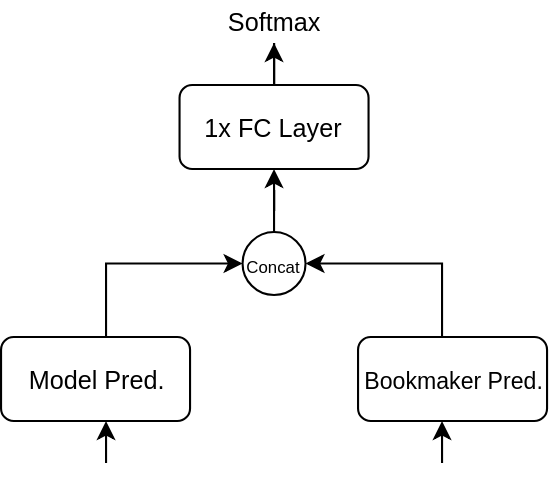
\includegraphics[scale=0.28]{img/Siamese3.png}
\caption{Refining bookmaker odds with our model predictions.}
\label{fig:oddsref}
\end{figure}


\begin{table}
\begin{tabular}{|c|c|}
\hline 
\textbf{Model} & \textbf{Accuracy} \\ 
\hline 
\hline 
Baseline (Bookmaker) & 0.51 \\ 
\hline 
FC Net & 0.49 \\ 
\hline 
Recurrent Net & 0.51 \\ 
\hline 
Odds Refinement with FC Net & 0.51 \\ 
\hline 
Odds Refinement with Recurrent Net & 0.52 \\ 
\hline 
\end{tabular} 
\label{tab:accs}
\caption{Results for the different models as evaluated on the test set.}
\end{table}


\subsection{Evaluation}
The results for our models on the test set can be found in Table \ref{tab:accs},
the fully connected network reaches 0.49 testing accuracy and the recurrent
model reaches 0.51 accuracy. Also we tested two additional models that use
bookmaker data as additional input where we fuse the predictions given by the
bookmakers and the predictions given by our models to try to refine the
bookmaker predictions (odds refinement in Table \ref{tab:accs}). We combine both
predictions in a single layer with Softmax activations, as depicted in
\ref{fig:oddsref} and train it with the same hyperparameters as the original
models. \\
One major problem we encountered was that the models basically never predict
draws as shown in their confusion matrices in Table \ref{tab:conffc} and
\ref{tab:confrnn}, we only saw draw predictions in heavily overfitted models but
these perform significantly worse on the other labels. Note that draws were the
least common result in our dataset and also bookmakers did not perform better on
predicting them than our models, on the test set they also basically never
predicted draws (on the whole data set they only predict draws a couple of
times), Table \ref{tab:confbm} depicts the confusion matrix of the betting
provider \textit{bet365} as evaluated on our test set.

\begin{table}
\begin{tabular}{|c||c|c|c|}
\hline 
 & pred home win & pred draw  & pred away win \\ 
\hline 
\hline
home win & 0.33 & 0.00 & 0.12 \\ 
\hline 
draw & 0.16 & 0.00 & 0.10 \\ 
\hline 
away win & 0.13 & 0.00 & 0.16 \\ 
\hline 
\end{tabular} 
\caption{Confusion matrix for the fully connected model evaluated on the test set.}
\label{tab:conffc}
\end{table}


\begin{table}
\begin{tabular}{|c||c|c|c|}
\hline 
 & pred home win & pred draw  & pred away win \\ 
\hline 
\hline
home win & 0.38 & 0.00 & 0.06 \\ 
\hline 
draw & 0.20 & 0.00 & 0.06 \\ 
\hline 
away win & 0.18 & 0.00 & 0.13 \\ 
\hline 
\end{tabular} 
\caption{Confusion matrix for the recurrent model evaluated on the test set.}
\label{tab:confrnn}
\end{table}


\begin{table}
\begin{tabular}{|c||c|c|c|}
\hline 
 & pred home win & pred draw  & pred away win \\ 
\hline 
\hline
home win & 0.39 & 0.00 & 0.06 \\ 
\hline 
draw & 0.19 & 0.00 & 0.07 \\ 
\hline 
away win & 0.16 & 0.00 & 0.13 \\ 
\hline 
\end{tabular} 
\caption{Confusion matrix for the bookmaker BW365 evaluated on the test set.}
\label{tab:confbm}
\end{table}

\FloatBarrier

\section{Conclusion}
\label{conclusion}
Prediciting football games is a very popular and challenging task. People
already tried to apply a broad range of different machine learning algorithms
and techniques to accurately predict the outcome of upcoming football games.
Even for humans it is very hard to predict whether the home team wins, the away
team wins or the game ends with a draw. The accuracy of humans and machine
learning approaches show that there are much more factors which have an impact
on the outcome of a football game. Maybe in-depth data-collection and
data-engineering can improve the prediction accuracy, sometimes it might even be
\textit{luck} if a team wins or loses.
\\\\
It is indisputable that there will be a lot of contributions in the context of
predicting football games in the future. A lot of people are fascinated by
sports and the betting industry generates high profits. For that reason there
will always be interest in this topic. It remains to be seen if new machine
learning approaches and more data are able to boost the performance of
computer-based prediction further and if neural networks are able to beat the
accuracy of human predictions permanently.

\bibliographystyle{IEEEtran}
\bibliography{report}

\end{document}

